%!TEX root = ../thesis.tex
%*******************************************************************************
%****************************** Third Chapter **********************************
%*******************************************************************************
\chapter{Deep neural networks for predicting DNA methylation} \label{sec:dcpg}

% **************************** Define Graphics Path **************************
\ifpdf
    \graphicspath{{Chapter4/Figs/Raster/}{Chapter4/Figs/PDF/}{Chapter4/Figs/}}
\else
    \graphicspath{{Chapter4/Figs/Vector/}{Chapter4/Figs/}}
\fi

Protocols for profiling DNA methylation in single cells are powerful for studying intercellular differences. However, they are limited by incomplete CpG coverage, which renders downstream analyses challenging. We therefore developed a deep neural network, \emph{DeepCpG}, for imputing incomplete DNA methylation profiles in single cells. In this chapter, we will describe the architecture of DeepCpG and show that it yields considerably more accurate predictions than existing methods across alternative cell types and sequencing protocols. In \cref{sec:dcpg_ana}, we will then present methods for analysing DNA methylation in single cells using DeepCpG. The presented work is based on \citet{angermueller_accurate_2017}.


\section{Motivation}

Single-cell DNA profiling technologies enabled the fine-grained study of DNA methylation in single cells. However, neither genome-wide (scBS-seq; \Cref{sec:bs}) nor reduced representation (scRRBS-seq; \Cref{sec:intro_proto}) protocols cover all CpG sites per cell. scBS-seq is limited by its efficiency to capture DNA and read-mapping biases, resulting in a CpG coverage of 10-30\% per cell. scRRBS-seq is limited to genomic regions of high CpG density by design, resulting in a CpG coverage of 1-10\% per cell. Unlike scBS-seq, scRRBS-seq is systematically biased towards CpG dense regions, making it impossible to obtain genome-wide CpG coverage by pooling cells.

The low CpG coverage renders several downstream analyses challenging, for example quantifying DNA methylation variability between cells (\Cref{sec:bs_method}), clustering cells (\Cref{sec:bs_method}), or correlating DNA methylation with gene expression. Whereas data of low CpG coverage can already be sufficient to reliably estimate average DNA methylation levels in large or CpG dense regions such as gene bodies or CGIs, analysing small or CpG poor regions is challenging. This holds true for many functional relevant regions such as enhancers or repressors, which we have found to be associated with high methylation variability between cells (\Cref{sec:bs_results}) and to be linked with changes in gene expression levels (\Cref{sec:mt_results}).

Methods for imputing incomplete DNA methylation profiles are therefore critical for analysing CpG methylation genome-wide.


\section{Existing methods and limitations}

While the problem of imputing single-cell methylation profiles has previously not been considered, methods have been developed for imputing average methylation levels in bulk populations of cells.

Some of these methods restrict predictions to a particular genomic context, for example CGIs. The methylation level of CGIs is relatively easy to predict since they are mainly hypomethylated, unlike the rest of the genome, which is mainly hypermethylated in somatic cells. For example, \citet{bock_cpg_2006} trained a support vector machine on DNA sequence-derived features and context annotations to predict CGI methylation in human lymphocytes. In addition to DNA sequence-derived features, \citet{zheng_cpgimethpred:_2013} found histone methylation- and histone acetylation marks to be important for predicting CGI methylation in multiple cell types.

Predicting methylation of individual CpG sites is more challenging since their methylation levels can vary considerably both within and across genomic contexts. For example, gene promoters that are overlapped by a CGI (CGI promoters) tend to be hypomethylated at the centre but hypermethylated at flanking regions, resulting in a bimodal distribution of methylation levels. In contrast, non-CGI promoters are mainly hypermethylated and can have alternative methylation patterns. Existing methods usually represent the methylation state of a CpG site as a binary or continuous variable, and use features extracted from the local neighbourhood of the CpG site to train a conventional machine learning classifier, such as logistic regression, support vector machine, random forest, na\"ive Bayes, or k-nearest neighbour. Features can be categorized into i) DNA sequence features, including the frequency of k-mers in a window centred on the target CpG site, GC-content, transcription factor binding sites, DNA conservation, single nucleotide polymorphism, and repeat elements, ii) context annotations, such as the type and function of nearby genomic regions, iii) structural information, including predicted structural elements and nucleosome positioning information, iv) histone modification marks, including histone methylation- and histone acetylation marks, and v) information about observed neighbouring CpG sites. For example, \citet{malousi_predictive_2014} trained a support vector machine only using DNA sequence features, including the frequency of di- and trinucleotides in 401~bp windows, known DNA sequence motifs, and Fourier-extracted periodicity signals. \citet{zhang_predicting_2015} proposed a random forest classifier trained on DNA sequence features, transcription factor binding sites, histone modification marks, as well as the methylation state and distance of the two closest neighbouring CpG sites.

To reduce the number of features and understand which features have the strongest influence on methylation levels, feature selection methods have been applied, including principal component analysis (\citep{zheng_enhancement_2011,zheng_cpgimethpred:_2013}), maximum-relevant-minimum redundancy (\citep{lu_predicting_2010}), sequential minimization optimization (\citep{malousi_predictive_2014}), and genetic algorithms~\citep{li_prediction_2014}.

Although existing methods have helped to better characterise DNA methylation in bulk populations of cells, they have multiple limitations. First, they separate feature extraction from model training. Instead of learning features from the raw data directly, features are pre-defined and manually extracted before model training. This makes it hard to discover new features since it is often a priori unclear which features are most relevant for predicting DNA methylation. Furthermore, feature extraction can be time-consuming and certain features might be unavailable for the cell type of interest. Second, most existing methods predict methylation for a single methylation profile without taking correlations between methylation profiles into account, for example from multiple cells. However, sharing information between related methylation profiles can improve prediction accuracy, in particular in domains where the methylation level of CpG sites is missing in some cells but available in others. ChromImpute~\citep{ernst_large-scale_2015} is a notable exception, a method that uses information from multiple epigenomic profiles, which, however, was not explicitly designed to predict DNA methylation. Third, some conventional machine learning models scale poorly to large datasets and cannot be trained online, which makes it impossible to adapt pre-trained models on new data. Some methods further do not support training on multiple tasks with missing labels, which is required for learning models on multiple cells with partially observed methylation levels.


\section{DeepCpG model architecture} \label{sec:dcpg_model}

To address the aforementioned limitations, we developed DeepCpG, a computational method based on deep neural networks (\Cref{sec:dl}) for predicting single-cell methylation states and for modelling the sources of DNA methylation variability. DeepCpG leverages associations between DNA sequence patterns and methylation states, as well as between neighbouring CpG sites, both within individual cells and across cells. Unlike previous methods~\citep{bhasin_prediction_2005,li_prediction_2014,liu_idna-methyl:_2015,lu_predicting_2010,stevens_estimating_2013,zhang_predicting_2015,zhou_prediction_2012}, DeepCpG does not separate the extraction of informative features and model training. Instead, DeepCpG is based on a modular architecture and learns predictive DNA sequence- and methylation patterns in a data-driven manner. Furthermore, DeepCpG is trained by online gradient descent, which enables to efficiently adapt or `fine-tune' pre-trained models on new data.

\begin{figure}[htbp!]
\centering
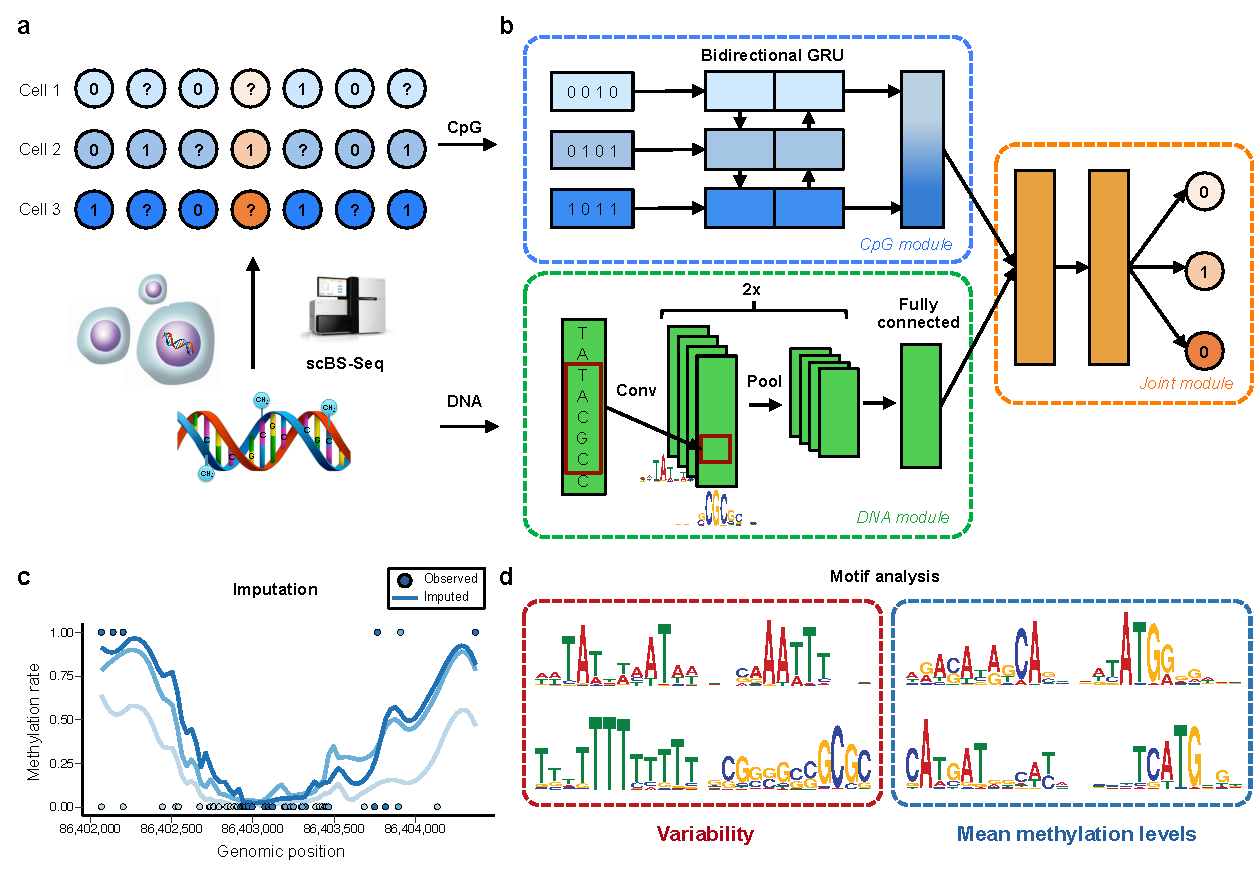
\includegraphics[width=1.0\textwidth]{method}
\caption[DeepCpG model training and applications.]{DeepCpG model training and applications. (a) Sparse single-cell CpG profiles as obtained from scBS-seq (\Cref{sec:bs}) or scRRBS-seq~\citep{farlik_single-cell_2015,guo_profiling_2015,hou_single-cell_2016}. Methylated CpG sites are denoted by ones, un-methylated CpG sites by zeros, and question marks denote CpG sites with unknown methylation state (missing data). (b) Modular architecture of DeepCpG. The DNA module consists of two convolutional and pooling layers to identify predictive motifs from the local sequence context, and one fully connected layer to model motif interactions. The CpG module scans the CpG neighbourhood of multiple cells (rows in b), using a bidirectional GRU (\Cref{sec:dl_rnn}), yielding compressed features in a vector of constant size. The joint module learns interactions between higher-level features derived from the DNA- and CpG module to predict methylation states in all cells. (c, d) The trained DeepCpG model can be used for different downstream analyses, including genome-wide imputation of missing CpG sites (c) and the discovery of DNA sequence motifs that are associated with DNA methylation levels or cell-to-cell variability (d).}
\label{fig:dcpg_method}
\end{figure}

DeepCpG predicts binary CpG methylation states from local DNA sequence windows and observed neighbouring methylation states (\Cref{fig:dcpg_method}~(a)). A major feature of the model is its modular architecture, consisting of a CpG module to account for correlations between CpG sites within and across cells, a DNA module to detect informative sequence patterns, and a joint module that integrates the evidence from the CpG and DNA module to predict methylation states at target CpG sites (\Cref{fig:dcpg_method}~(b)).


\subsection{DNA module}

The DNA module is a CNN (\Cref{sec:dl_cnn}) consisting of a stack of convolutional and pooling layers, which is followed by one fully connected hidden layer. CNNs are designed to extract features from high-dimensional inputs while keeping the number of model parameters tractable by applying a series of convolutional and pooling operations. Unless stated otherwise, the DNA module takes as input a 1001~bp long DNA sequence centred on a target CpG site $n$, which is represented as a binary matrix $s_n$ by one-hot encoding the $D=4$ nucleotides as binary vectors $A=[1, 0, 0, 0]$, $T=[0, 1, 0, 0]$, $G=[0, 0, 1, 0]$, and $C=[0, 0, 0, 1]$. The input matrix $s_n$ is first transformed by a one-dimensional convolutional layer, which computes the activation $a_{nfi}$ of multiple convolutional filters $f$ at every position $i$ within the DNA sequence window:
\begin{align} \label{eq:dcpg_filter_act}
  a_{nfi}=\operatorname{ReLU}(\sum_{l=1}^L \sum_{d=1}^D w_{fld} s_{n,i+l,d})
\end{align}
Here, $w_f$  are the parameters or weights of convolutional filter $f$ of length $L$. These can be interpreted similarly to position weight matrices, which are matched against the input DNA sequence window $s_n$ at every position $i$ to recognize distinct motifs. The $\operatorname{ReLU}(x)=\max(0,x)$ activation function sets negative values to zero, such that $a_{nfi}$ corresponds to the evidence that the motif represented by $w_f$ occurs at position $i$.

A pooling layer is used to summarize the activations of $P$ adjacent neurons by their maximum value:
\begin{align}
  p_{nfi}=\max_{|k|<P/2}(a_{nf,i+k})
\end{align}
Non-overlapping pooling is applied with step size $P$ to decrease the dimension of the input sequence and hence the number of model parameters. The DNA module has multiple pairs of convolutional-pooling layers to learn higher-level interactions between sequence motifs, which are followed by one final fully connected layer with a ReLU activation function. The number of convolutional-pooling layers is a hyperparameter, which was selected by optimizing the prediction performance on the validation set (\Cref{sec:dl_hyper}).


\subsection{CpG module}

The CpG module consists of a non-linear embedding layer to model dependencies between CpG sites within cells, which is followed by a bidirectional GRU (\Cref{sec:dl_rnn}) to model dependencies between cells. Inputs are $100d$ vectors $x_1,\ldots,x_T$, where $x_t$ represents the methylation state and distance of $K=25$ CpG sites to the left and to the right of a target CpG site in cell $t$. Distances were transformed to relative ranges by dividing by the maximum genome-wide distance. The embedding layer is fully connected and transforms $x_t$ into a $256d$ vector $\bar{x}_t$, which allows learning possible interactions between methylation states and distances within cell $t$:
\begin{align}
  \bar{x}_t=\operatorname{ReLU} (W x_t + b)
\end{align}
The sequence of vectors $\bar{x}_t$ are then fed into a bidirectional GRU, which scans input sequence vectors $\bar{x}_1,\ldots,\bar{x}_T$ from left to right, and encodes them into fixed-size hidden state vectors $h_1,\ldots,h_T$:
\begin{align}
  &r_t=\operatorname{sigmoid}(W_{rx} \bar{x}_t + W_{rh} h_{t-1} + b_{r}) \nonumber \\
  &u_t=\operatorname{sigmoid}(W_{ux} \bar{x}_t + W_{uh} h_{t-1} + b_{u}) \nonumber \\
  &\tilde{h}_t=\operatorname{tanh}\left(W_{\tilde{h}x} \bar{x}_t + W_{\tilde{h}h}(r_t \odot h_{t-1}) + b_{\tilde{h}}\right) \nonumber \\
  &h_t = (1 - u_t) \odot h_{t-1} + u_t \odot \tilde{h}_t
\end{align}
The reset gate $r_t$ and update gate $u_t$ determine the relative weight of the previous hidden state $h_{t-1}$ and the current input $\bar{x}_t$ for updating the current hidden state $h_t$. The last hidden state $h_T$ summarizes the sequence as a fixed-size vector. Importantly, the set of parameters $W$ and $b$ are independent of the sequence length $T$, which enables to fine-tune a pre-trained CpG module on a new dataset with a different number of cells.

By using a bidirectional GRU, cell-to-cell dependencies are encoded independently of the order of cells. It consists of a forward and backward GRU with $256d$ hidden state vectors $h_t$, which scan the input sequence from the left and right, respectively. The last hidden state vector of the forward and backward GRU are concatenated into a $512d$, which forms the output of the CpG module.


\subsection{Joint module}

The joint module takes as input the concatenated last hidden vectors of the DNA and CpG module, and models interactions between the extracted DNA sequence and CpG neighbourhood features via two fully connected hidden layers with 512 neurons and ReLU activation function. This enables context-dependent smoothing of neighbouring CpG sites and hence modelling of alternatively shaped methylation profiles, for example in promoter or enhancer regions. The output layer of the joint module contains $T$ sigmoid neurons to predict the methylation rate $\hat{y}_{nt}\in(0;1)$ of CpG site $n$ in cell $t$:
\begin{align} \label{eq:dcpg_y}
  \hat{y}_{nt}=\operatorname{sigmoid}(x)=\frac{1}{1+e^{-x}}
\end{align}


\subsection{Model training}

Model parameters were learned on the training set by minimizing the following loss function:
\newcommand{\Xnll}{\operatorname{NLL}_w(\hat{y},y)}
\begin{align}
  L(w)=\Xnll+\lambda_2 \norm{w}_2
\end{align}
Here, the weight-decay hyperparameter $\lambda_2$ penalises large model weights quantified by the L2 norm, and $\Xnll$ denotes the negative log-likelihood, which measures how well the predicted methylation rates $\hat{y}_{nt}$ fit to observed binary methylation states $y_{nt}\in\{0,1\}$:
\begin{align}
  \Xnll=\sum_{n=1}^N \sum_{t=1}^T o_{nt}\left[y_{nt} \log(\hat{y}_{nt}) + (1-y_{nt}) \log(1-\hat{y}_{nt})\right]
\end{align}
The binary indicator $o_{nt}$ is set to one if the methylation state $y_{nt}$ is observed for CpG site $n$ in cell $t$, and zero otherwise. Dropout (\citep{srivastava_dropout:_2014}; \Cref{sec:dl_overfit}) with different dropout rates for the sequence, CpG, and joint module was used for additional regularization. Model parameters were initialized randomly following the approach in \citet{glorot_understanding_2010}. The loss function was optimized by mini-batch stochastic gradient descent with a batch size of 128 and a global learning rate of 0.0001. The learning rate was adapted by Adam (\citep{kingma_adam:_2014}; \Cref{sec:dl_adapt}), and decayed by a factor of 0.95 after each epoch. Learning was terminated if the validation loss did not improve over ten consecutive epochs (early stopping). The DNA and CpG module were pre-trained independently to predict methylation from the DNA sequence (DeepCpG DNA) or the CpG neighbourhood (DeepCpG CpG). For training the joint module, only the parameters of the hidden layers and the output layers were optimized, whiling keeping the parameters of the pre-trained DNA and CpG module fixed. Training DeepCpG on 18 serum mESCs using a single NVIDIA Tesla K20 GPU took approximately 24 hours for the DNA module, 12 hours for the CpG module, and 4 hours for the joint module. Model hyperparameters were optimized on the validation set by random sampling (\citep{bengio_practical_2012}; \Cref{sec:dl_hyper}).


\subsection{Software availability}

DeepCpG is publicly available on Github\footnote{\url{https://github.com/cangermueller/deepcpg}} and implemented in Python using Theano~\citep{bastien_theano:_2012} and Keras~\citep{chollet_keras:_????}. Our software includes documentation and interactive tutorials on training, evaluating, and analysing DeepCpG. We also provide pre-trained models, which can be efficiently fine-tuned on new data.


\section{Prediction performance evaluation} \label{sec:dcpg_eval}

First, we assessed the ability of DeepCpG to predict single-cell methylation states and compared the model to existing imputation strategies for DNA methylation. As a baseline approach, we considered local averaging of the observed methylation states, either in 3 kb windows centred on the target site of the same cell (WinAvg; \Cref{sec:bs_method}) or across cells at the target site (CpGAvg). Additionally, we compared DeepCpG to a random forest classifier~\citep{breiman_random_2001} trained on individual cells using the DNA sequence information and neighbouring CpG states as input (RF). Finally, we evaluated a recently proposed random forest classifier for predicting methylation rates in bulk populations of cells~\citep{zhang_predicting_2015}, which takes comprehensive DNA annotations into account, including genomic contexts, and tissue-specific regular annotations, such as DNase1 hypersensitivity sites, histone modification marks, and transcription factor binding sites (RF Zhang). All methods were trained, selected, and tested on distinct chromosomes via holdout validation (\Cref{sec:dl_eval}). Specifically, we used chromosomes 1, 3, 5, 7, 9, and 11 as training set, chromosomes 2, 4, 6, 8, 10, and 12 as test set, and the remaining chromosomes as validation set. For each cell type, models were fit on the training set, hyperparameters were optimized on the validation set, and the final model performance and interpretations were exclusively reported on the test set.

Since the proportion of methylated versus unmethylated CpG sites can be unbalanced in globally hypo- or hypermethylated cells, we used the area under the receiver operating characteristics curve (AUC) to quantify the prediction performance of different models. We have also considered a range of alternative metrics, including precision-recall curves, F1 score~\citep{powers_evaluation:_2011}, and Matthews correlation coefficient~\citep{matthews_comparison_1975}, resulting in overall consistent conclusions (\Cref{fig:dcpg_eval_curves}; \Cref{fig:dcpg_eval_dsets_all}).

Initially, we applied all methods to 18 serum-cultured mouse embryonic stem cells (mESCs; average CpG coverage 17.7\%; \Cref{fig:dcpg_eval_cells}), profiled using scBS-seq (\Cref{sec:bs}).

\begin{figure}[htbp!]
\centering
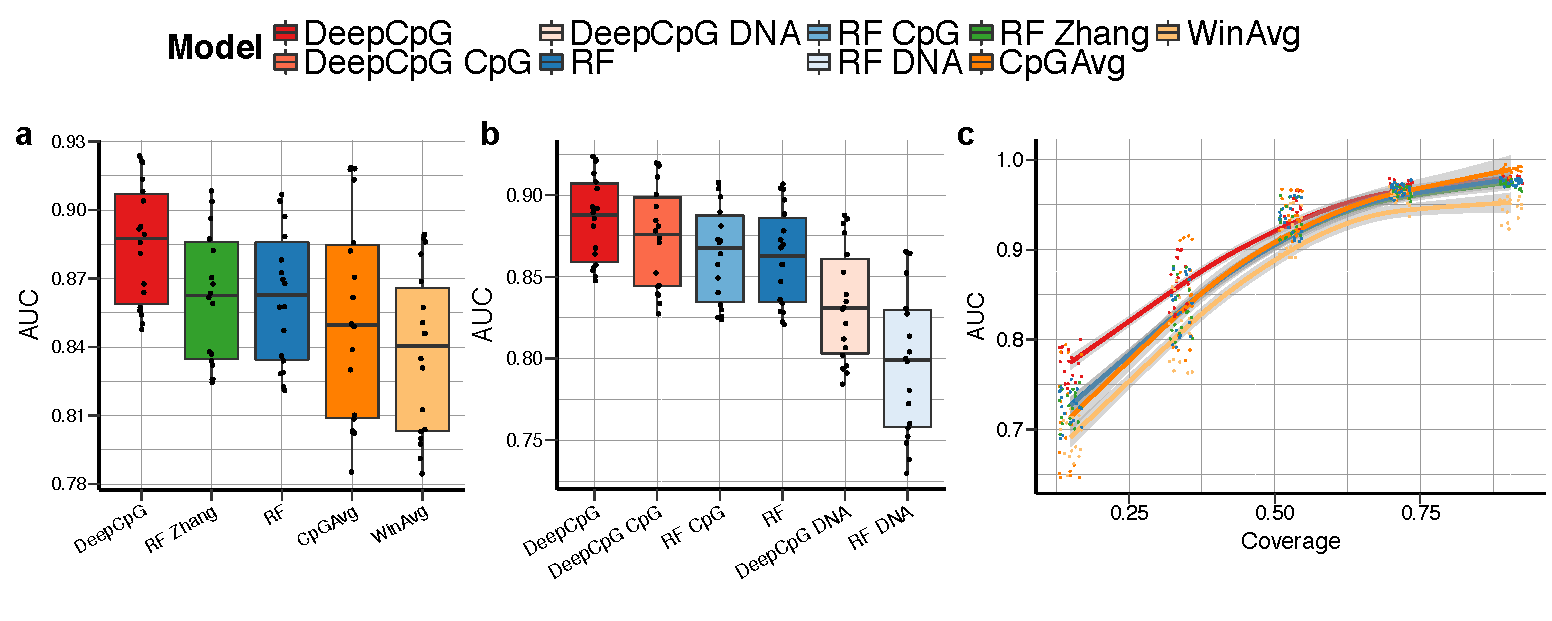
\includegraphics[width=1.0\textwidth]{eval_global}
\caption[Prediction performance of DeepCpG.]{Prediction performance of DeepCpG. (a) Genome-wide prediction performance for 18 serum-grown mouse embryonic stem cells (mESCs) profiled using scBS-seq. Performance is measured by the area under the receiver-operating characteristic curve (AUC), using holdout validation. Considered were DeepCpG, random forest classifiers trained either using DNA sequence and CpG features (RF) or trained using additional annotations from corresponding cell types (RF Zhang). Additionally, two baseline methods were considered, which estimate methylation states by averaging observed methylation states, either across consecutive 3 kb regions within individual cells (WinAvg) or across cells at a single CpG site (CpGAvg). (b) Performance breakdown of DeepCpG and RF, comparing the full models to models trained either only using methylation features (DeepCpG CpG, RF CpG) or DNA features (DeepCpG DNA, RF DNA). (c) AUC of the methods as in (a) stratified by genomic contexts with increasing CpG coverage across cells. Trend lines were fit using local polynomial regression (LOESS); shaded areas denote 95\% confidence intervals.}
\label{fig:dcpg_eval}
\end{figure}

DeepCpG yielded more accurate predictions than any of the alternative methods, both genome-wide and in different genomic contexts (\Cref{fig:dcpg_eval}). Notably, DeepCpG was consistently more accurate than RF Zhang, a model that relies on genomic annotations. These results indicate that DeepCpG can automatically learn higher-level features from the DNA sequence. To investigate this, we tested for associations between the activity of convolutional filters in the DNA module and known sequence annotations (\Cref{sec:dcpg_ana_motifs}), finding both positive and negative correlations with several annotation contexts, including DNase1 hypersensitive sites, histone modification marks, and CpG-rich genomic contexts (\Cref{fig:dcpg_eval_motifs_feat}). The ability to extract higher-level features from the DNA sequence is particularly important for analysing single-cell datasets, where individual cells may be from different cell types and states, making it difficult to derive appropriate annotations.

To assess the relative importance of DNA sequence features compared to neighbouring CpG sites, we trained the same models, however, either exclusively using DNA sequence features (DeepCpG DNA, RF Seq) or neighbouring methylation states (DeepCpG CpG, RF CpG). Consistently with previous studies in bulk populations~\citep{zhang_predicting_2015}, methylation states were more predictive than DNA features, and models trained with both CpG and DNA features performed best (\Cref{fig:dcpg_eval}~(b)). Notably, DeepCpG trained with CpG features alone outperformed a random forest classifier trained with both CpG and DNA features. A likely explanation for the accuracy of the CpG module is its recurrent network architecture, which enables the module to effectively transfer information from neighbouring CpG sites across different cells (\Cref{fig:dcpg_eval_cpg_module}).

\begin{figure}[htbp!]
  \begin{minipage}[c]{0.65\textwidth}
    \centering
    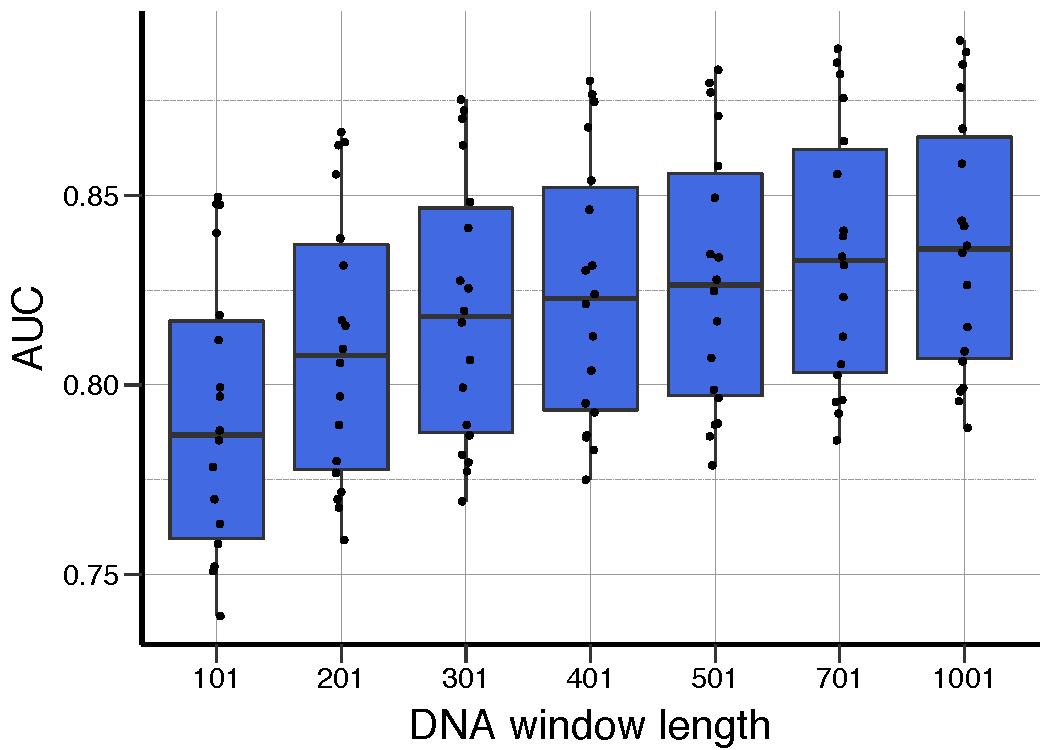
\includegraphics[width=1.0\textwidth]{dna_module_wlen}
  \end{minipage}
  \begin{minipage}[c]{0.32\textwidth}
    \caption[Prediction performance of the DeepCpG DNA module for DNA sequence windows of increasing length.]{Prediction performance of the DeepCpG DNA module for DNA sequence windows of length 101~bp up to 1001~bp.}
    \label{fig:dcpg_eval_dna_module_wlen}
  \end{minipage}
\end{figure}

The largest relative gains between RF and DeepCpG were observed when training both models with DNA sequence information only (AUC 0.83 versus 0.80; \Cref{fig:dcpg_eval}~(b)). This demonstrates the strength of the DeepCpG DNA module to extract predictive sequence features from large DNA sequence windows of up to 1001~bp (\Cref{fig:dcpg_eval_dna_module_wlen}), which is in particular critical for accurate predictions from DNA in uncovered genomic regions, for example when using reduced representation sequencing data~\citep{farlik_single-cell_2015,guo_single-cell_2013,hou_single-cell_2016}. Consistent with this, the relative performance gain of DeepCpG compared to other methods was highest in contexts with low CpG coverage (\Cref{fig:dcpg_eval}~(c); \Cref{fig:dcpg_eval_stats}).

\begin{figure}[htbp!]
\centering
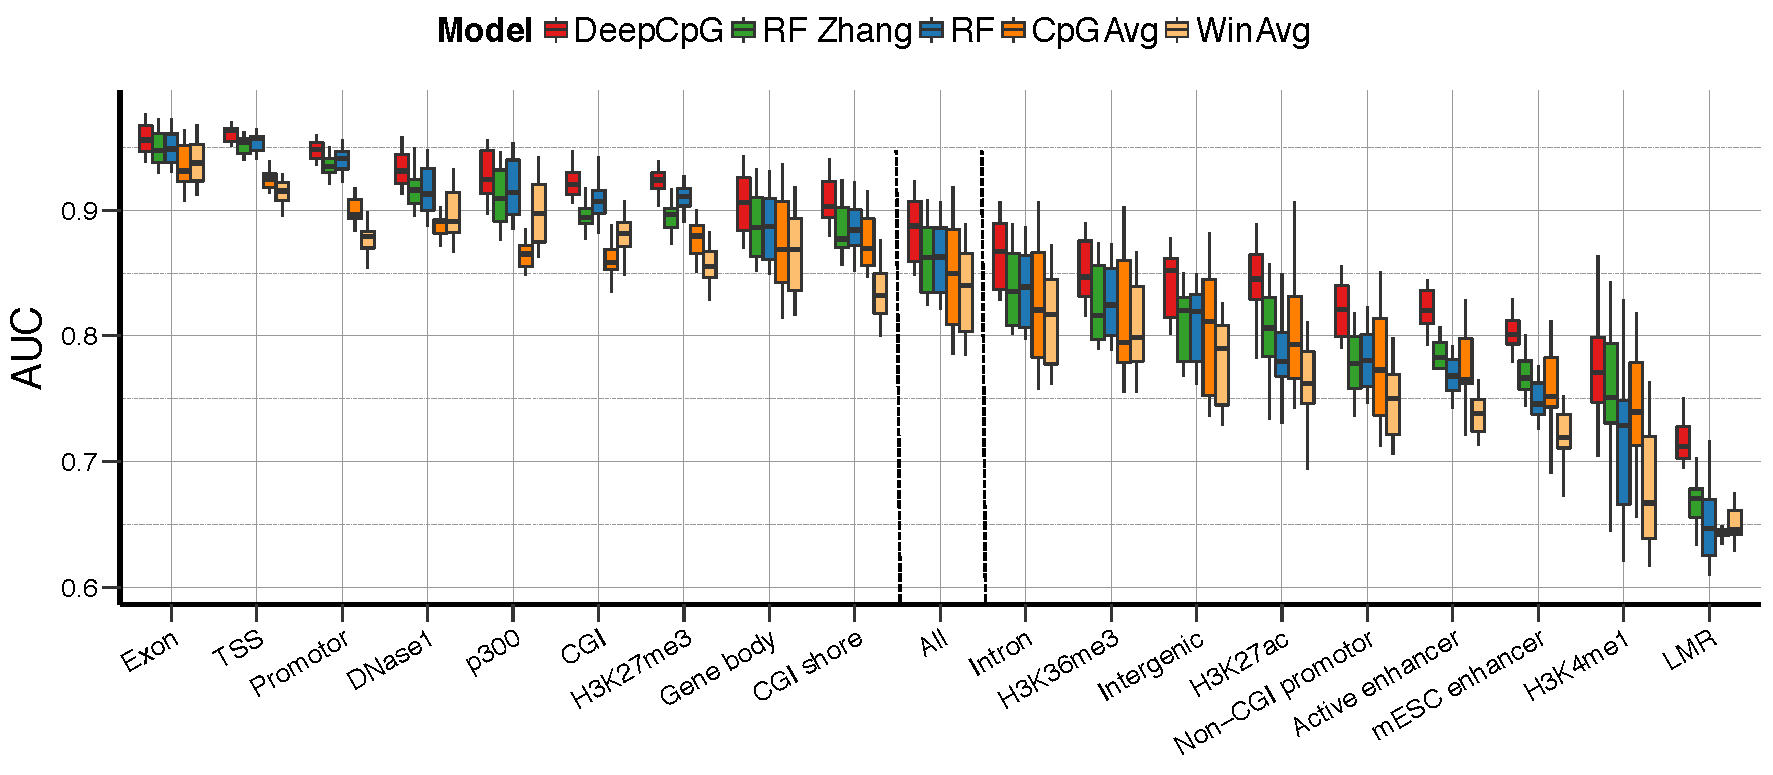
\includegraphics[width=1.0\textwidth]{eval_annos}
\caption[Prediction performance of DeepCpG for alternative genomic contexts.]{Prediction performance of DeepCpG for alternative genomic contexts, with `All' corresponding to genome-wide performances.}
\label{fig:dcpg_eval_annos}
\end{figure}

Next, we explored the prediction performance of all models in different genomic contexts. In line with previous findings~\citep{stevens_estimating_2013,zhang_predicting_2015}, all models performed best in GC-rich contexts (\Cref{fig:dcpg_eval_annos}). However, DeepCpG offered most advantages in GC-poor genomic contexts, including non-CGI promoters, enhancer regions, and histone modification marks (H3K4me1, H3K27ac)--contexts that we found to be associated with higher methylation variability between cells (\Cref{sec:bs_results}).

\begin{figure}[htbp!]
\centering
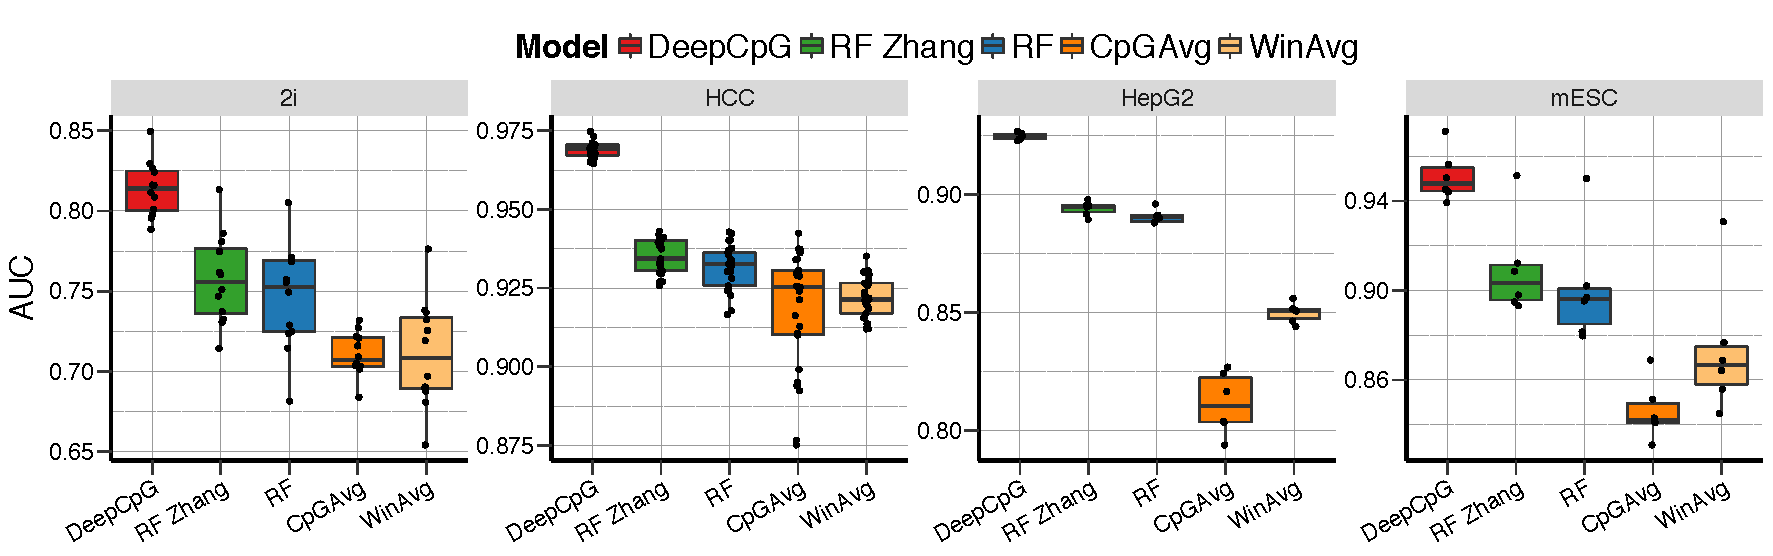
\includegraphics[width=1.0\textwidth]{eval_dsets}
\caption[Prediction performance of DeepCpG for alternative datasets.]{Prediction performance of DeepCpG for alternative datasets. Shown are genome-wide performances for 12 2i-grown mESCs profiled using scBS-seq, as well as three cell types profiled using scRRBS-seq, including 25 human HCC cells, 6 HepG2 cells, and 6 additional mESCs.}
\label{fig:dcpg_eval_dsets}
\end{figure}

We also applied DeepCpG to 12 2i-cultured mESCs profiled using scBS-seq and to data from three cell types profiled using scRRBS-seq~\citep{hou_single-cell_2016}, including 25 human hepatocellular carcinoma cells (HCC), 6 human heptoplastoma-derived (HepG2) cells, and an additional set of 6 mESCs. Notably, in contrast to the serum cells, the human cell types are globally hypomethylated (\Cref{fig:dcpg_eval_cells}). Across all cell types, DeepCpG yielded substantially more accurate predictions than alternative methods (\Cref{fig:dcpg_eval_dsets}; \Cref{fig:dcpg_eval_dsets_all}), demonstrating the broad applicability of the model, including to hypo- and hypermethylated cells, as well to data generated using different sequencing protocols.


\section{Discussion}

We have developed a deep neural network, \emph{DeepCpG}, for predicting DNA methylation in single cells. We have demonstrated that our model enables accurate imputation of missing methylation states, thereby facilitating genome-wide downstream analyses. DeepCpG offers major advantages in shallow sequenced cells as well as in sparsely covered sequence contexts with increased methylation variability between cells. Our method may also help to reduce the required sequencing depth in single-cell bisulfite sequencing studies, thereby enabling the analysis of larger numbers of cells at reduced cost.

The increased accuracy of DeepCpG comes at the expense of higher compute costs. Training DeepCpG genome-wide on a single GPU takes about two days, which is considerably longer compared with conventional machine learning models. However, parallelising computations across multiple GPUs and compute nodes can drastically reduce the training time. Since DeepCpG processes all cells simultaneous, it further shares computations across cells and hence scales better than existing methods to data sets with many cells. Faster training is also possible by only fine-tuning a model that was pre-trained on a related cell type instead of training a new model from scratch.

An important area of future work is to simultaneously impute multiple bulk and single-cell methylation profiles, and to integrate different data modalities from parallel-profiling methods, which are now becoming increasingly available for multiple molecular layers.
